\documentclass[12pt,letterpaper,spanish]{article}
\usepackage[spanish]{babel}
\usepackage[utf8]{inputenc}
\usepackage{times}
\usepackage{amsmath}
\usepackage{amsfonts}
\usepackage{amssymb}
\usepackage{titlesec}
\usepackage[left=2.54cm,right=2.54cm,top=2.54cm,bottom=2.54cm]{geometry}
\title{Diseño e implementación de una unidad electroquirúrgica 
enfocada en la reducción del volumen de pérdida de sangre}
\usepackage{graphicx}
\usepackage{float}
\usepackage{textgreek}
\setcounter{secnumdepth}{5}
\renewcommand{\baselinestretch}{2}

\titleformat{\section}[hang]{\filcenter\bfseries}{\thesection.}{1cm}{}
\titleformat{\subsection}[hang]{\filright\bfseries}{\thesubsection.}{0.5cm}{}
\titleformat{\subsubsection}[hang]{\filright\bfseries}{\thesubsubsection.}{0.5cm}{}
\titleformat{\paragraph}[hang]{\filright\bfseries\itshape}{\theparagraph.}{0.5cm}{}


\begin{document}
	\tableofcontents
	\newpage
	
	\section{Introducción}
	La Ingeniería Electrónica es la rama de la Física que mediante el aprovechamiento de fenómenos electromagnéticos y el comportamiento de las cargas eléctricas, se aplican soluciones teóricas y practicas a una amplia gama de problemáticas. En particular el proyecto aprovecha la capacidad de aplicar tecnologías novedosas en el ámbito de los organismos biológicos, para combinarlas y de este modo obtener un producto que mejore la calidad de vida, humana o de procedencia animal.       	
	
		\subsection{La Bioingeniería}
		La Bioingeniería es un campo que combina los conocimientos del área ingenieril con la ciencia que se dedica a estudiar los seres vivos, es decir, la biología. Posee un amplio espectro de desarrollo, en donde encontramos diversas especialidades, tales como la ingeniería genética, la biomimética o la biomédica, esta ultima en concreto, sienta las bases necesarias para la elaboración de la unidad electroquirúrgica 
enfocada en la reducción del volumen de pérdida de sangre.   		
			
		\subsection{La Ingeniería Biomédica}
		La especialidad en la cual se desenvuelve el proyecto es denominada ingeniería biomédica, su concepto se basa en el estudio de campos derivados del cuidado de la salud, como lo son la medicina, odontología, veterinaria, la fisiología entre otros, y su finalidad es utilizar soluciones practicas a
dichos campos, por medio de el conocimiento teórico y empírico previamente adquirido. La biomédica ha estado vigente durante algunas décadas, no obstante es un tema relativamente nuevo para el entorno nacional, no solo hablando en términos de venta y distribución de la tecnología existente sino también para la innovación y desarrollo de nuevos dispositivos.
		
			\subsubsection{Ingeniería Biomédica en Colombia y el Mundo}
						
			
			\subsubsection{La Electrocirugía}
			
	
	\section{Bases Teóricas}
	La complejidad del proyecto derivo en que la teoría presente en el desarrollo de este, sea por un lado fundamentación médica, la cual proporciona los parámetros de operabilidad del dispositivo, mientras por otra parte, el conocimiento empírico o técnico aporta una solución practica a estos requerimientos médicos establecidos.   	
	
		\subsection{Teoría Médica}
		
		
			\subsubsection{Efectos de la Corriente sobre el Cuerpo Humano}	
			Es prudente aclarar que el paso de electricidad sobre el cuerpo humano, dependiendo de su procedencia y la forma en la que se aplique, puede afectar de manera mas o menos severa la integridad de un ser vivo. Específicamente debemos tener en cuenta el efecto de la corriente alterna, basados en estudios previos, con motivo de limitar las características de aplicación sobre el paciente y estandarizar el equipo en producción.
			Como bien sabemos la corriente alterna posee dos características fundamentales que representan su comportamiento: la magnitud y la fase. Dentro de estos dos conceptos se sitúan las variables que podemos modificar      		
			
				\paragraph{Relación entre estimulo Eléctrico y la producción de un estímulo Neuro-Muscular }	
			\subsubsection{El Electrobisturí}
			
				\paragraph{Fundamentos Electroquirúrgicos}
				\paragraph{Características de la electrocirugía}
				\paragraph{Calculo de los parámetros para la electrocirugía}
			\subsubsection{La Electrocardiografía}
			\subsubsection{La Bioimpedanciometría}
			El sensado de impedancia dentro de los sistemas circuitales, es de vital importancia para la 	instrumentación de estos y por ende el correcto funcionamiento dentro del proceso requerido. Para obtener los valores de impedancia reales de un objeto en general se utilizan elementos como los empleados por los multímetros, basados en galvanómetros y resistencias de calibración [1], sin embargo para la obtención del valor de impedancia en un tejido biológico o bioimpedancia, existen elementos en particular que no solo realizan este procedimiento de manera efectiva, sino que tampoco comprometen el estado del ente involucrado en el proceso de medición.
			
				\paragraph{Impedancia Eléctrica de los Tejidos}
				\hfill\break
				La impedancia como tal  es la oposición de un material al flujo de corriente sobre este. Con la bioimpedancia esta afirmación no es una excepción, pero además se tiene que la condición de dichos tejidos determina directamente su capacidad conductiva y de almacenamiento de electricidad.
			
				\begin{figure}[H]
					\centering
					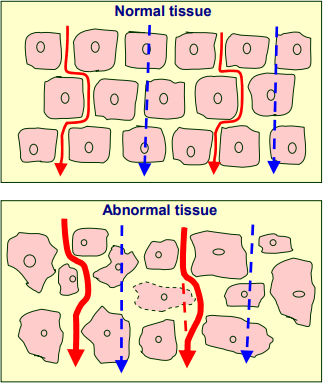
\includegraphics[width=0.5\textwidth]{./Imagenes/Tejido.png}
					\caption{Tipo de Tejido según su Condición}
				\end{figure}
			
				Así mismo la medida de bioimpedancia tiende a variar de acuerdo al tipo de tejido al cual nos estemos refiriendo. Es de tal modo, que por ejemplo la piel en su estructura completa posee un mayor valor de impedancia con respecto al tejido muscular, pero un valor inferior al tejido no magro o también llamado tejido graso.
				\paragraph{Tipos de Tejido}
				\hfill\break
				Para el ámbito en el cual nos encontramos, es decir, bioimpedancia, existen diversas formas de clasificar los tejidos, pero a groso modo, citaremos los analizados en el libro Bioimpedance and Bioelectricity Basics, para tomar valores de referencia con los cuales se podrá completar con ellos las calibración de los dispositivos utilizados en el presente modulo.
			
				\begin{itemize}
					\item Tejido Muscular o Magro.
					\item Tejido Nervioso.
				 	\item Tejido Adiposo o Graso y Tejido Óseo.
					\item Sangre.
				\end{itemize}
			
				\begin{figure}[H]
					\centering
					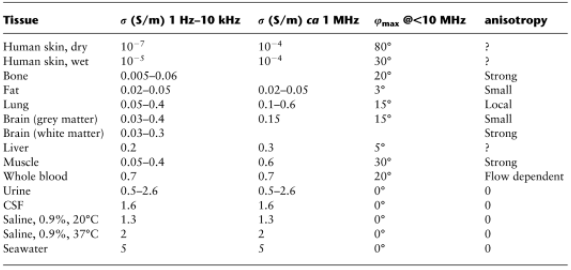
\includegraphics[width=0.7\textwidth]{./Imagenes/Imp_Tejido.png}
					\caption{Escala de Impedancia de los Tejidos}
				\end{figure}
			
				Aquí observamos claramente que existe una variación no solo con las características antes mencionadas, estado del tejido y tipo de tejido, sino también con la frecuencia a la que se realiza la caracterización del tejido. 
			
				Como sabemos la impedancia presente en el tejido vivo corresponde directamente con su capacidad conductiva, en ese sentido, elementos a nivel macroscópico y microscópico son responsables de su comportamiento ante una excitación eléctrica, entre estos elementos se encuentran la extensión del tejido, su nivel de hidratación tanto extra como intracelularmente hablando, temperatura, entre otros. Por ello los valores de impedancia que se obtienen al aplicar sobre estos tejido un flujo de corriente continua es de tipo capacitivo, esto implica, que además de la magnitud del dato arrojado habrá una fase.

				Esta es por tanto la base teórica de nuestro sistema, la adquisición de un dato imaginario y uno real, en donde a base de fórmulas aritméticas obtengamos con la mayor certeza posible la magnitud o valor resistivo del elemento o elementos sobre los cuales actuara el electrobisturí.

				\paragraph{Precauciones de Sensado}
				\hfill\break
				Como es bien sabido, la aplicación de corriente sobre el cuerpo humano, o cualquier ser vivo, debe conllevar una serie de precauciones necesarias para evitar efectos perjudiciales de salud. 
Como es citado en empresas especializadas en equipo médico, en este caso TÜV, incluso los niveles de corriente pequeños para las frecuencias de distribución usadas a nivel mundial, es decir, 50 y 60 Hz, pueden repercutir en daños clínicos irreversibles.
			
				\begin{figure}[H]
					\centering
					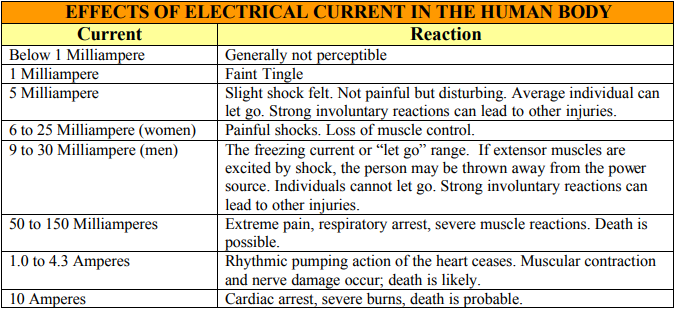
\includegraphics[width=0.9\textwidth]{./Imagenes/Current_Ef.png}
					\caption{Escala de Impedancia de los Tejidos}
				\end{figure}			
			
				El dispositivo elegido debe por lo tanto, no solo ser de carácter fiable, sino que a su vez procure trabajar con parámetros específicamente diseñados para el tratamiento de “Bioimpedancias”, en nuestro caso fue el circuito integrado AD5933.
			
				La razón de elección es su amplio rango de impedancias medibles (entre 100$\Omega$ y 10M$\Omega$) y la frecuencia de aplicación de sus señales de excitación (Frecuencia máxima recomendada de hasta 100KHz). Con la información previa recopilada podemos determinar que según la reglamentación de seguridad para equipos médicos en Colombia podemos acoplar este elemento al sistema final completo [5].
		
			\subsubsection{Seguridad Eléctrica en Equipos Médicos}	
				\paragraph{Clasificación de los Equipos Médicos según las Normas de Seguridad ICE}	
		
		\subsection{Teoría Técnica}
		
	\section{Diseño y Construcción del Electrobisturí}
		\subsection{Generador de Ondas}
		
		\subsection{Bioimpedanciometro}	
			\subsubsection{Características}
			En base al circuito integrado elegido, AD5933, se elabora un sistema que asegure una captación de datos de manera continua, con un margen de error mínimo, procurando reducir al máximo la interferencia generada por el ruido proveniente de los circuitos circundantes.
			
Es prudente aclarar que dentro del dispositivo en uso, está desarrollado un sistema de bloques propio, el cual se procederá a describir, más no a fondo, toda la documentación sin embargo esta disponible en la hoja de datos  presente en la página del fabricante.

			\begin{figure}[H]
				\centering
				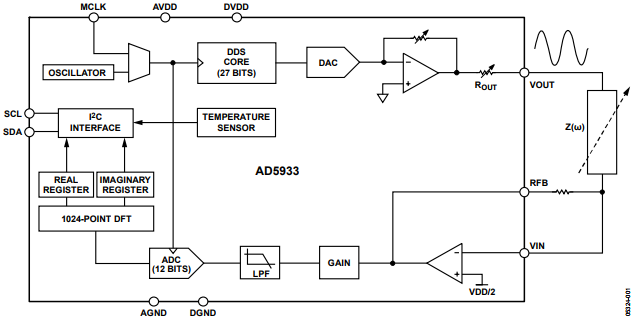
\includegraphics[width=0.7\textwidth]{./Imagenes/D_Bloques_AD5933.png}
				\caption{Diagrama de Bloques Interno, Circuito Integrado AD5933}
			\end{figure}
			
				\paragraph{Componentes}
				\hfill\break
				Además del circuito principal, basados en las recomendaciones del fabricante y para efecto de una implementación que permita trabajar en el rango establecido de impedancias para tejido animal, surge como guía el documento CN-0217, en donde es habilitado la escala entre 100$\Omega$ a 1K$\Omega$, que de otra forma el AD5933 no podría procesar individualmente [7]. 
				
			\begin{figure}[H]
				\centering
				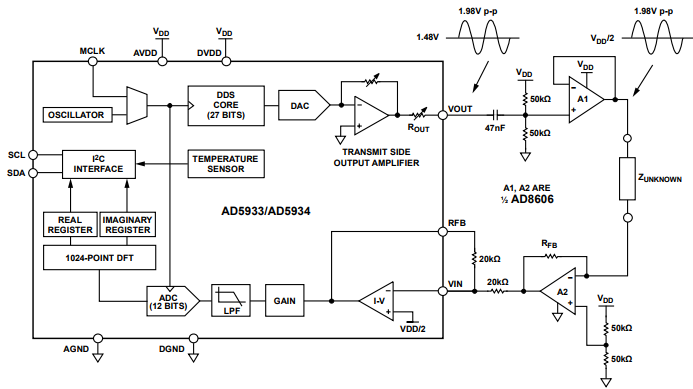
\includegraphics[width=0.7\textwidth]{./Imagenes/Bio_Circuito.png}
				\caption{Sistema Circuital Bioimpedanciometro}
			\end{figure}				
				
				El sistema circuital diseñado en esta sección busca un filtrado de la señal de DC, es decir, de las tensiones o corrientes de polarización y/o offset del IC, para evitar imprecisiones que incrementen el error entre datos teóricos y datos reales. 
Posterior a ello se utilizan amplificadores con configuración de buffer, en función de tener la impedancia más baja posible a la salida de dicho sistema.
Adicional a ello se utiliza una función de apoyo en donde se capta un primer dato de referencia que le indica al circuito el orden de las impedancias a sensar, disminuyendo en este sentido la posibilidad de grandes fluctuaciones de los datos recopilados. Para tal fin se selecciona una resistencia de calibración que se encuentre en una posición media en la escala de datos obtenibles.
			
			\begin{figure}[H]
				\centering
				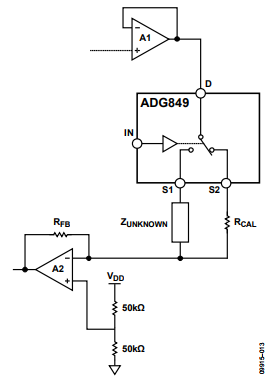
\includegraphics[width=0.5\textwidth]{./Imagenes/Anexo_Bio.png}
				\caption{Complemento Sensado de Bioimpedanciometría}
			\end{figure}
			
				\paragraph{Sistema de Bloques}
				\hfill\break
			Con todos los componentes mencionados previamente de manera de general, se procede a establecer el sistema de bloques donde se desglose de manera menos intuitiva el circuito de bioimpedanciometría. Con todos los componentes mencionados previamente de manera de general, se procede a establecer el sistema de bloques donde se desglose de manera menos intuitiva el circuito de bioimpedanciometría. 

				\begin{figure}[H]
					\centering
					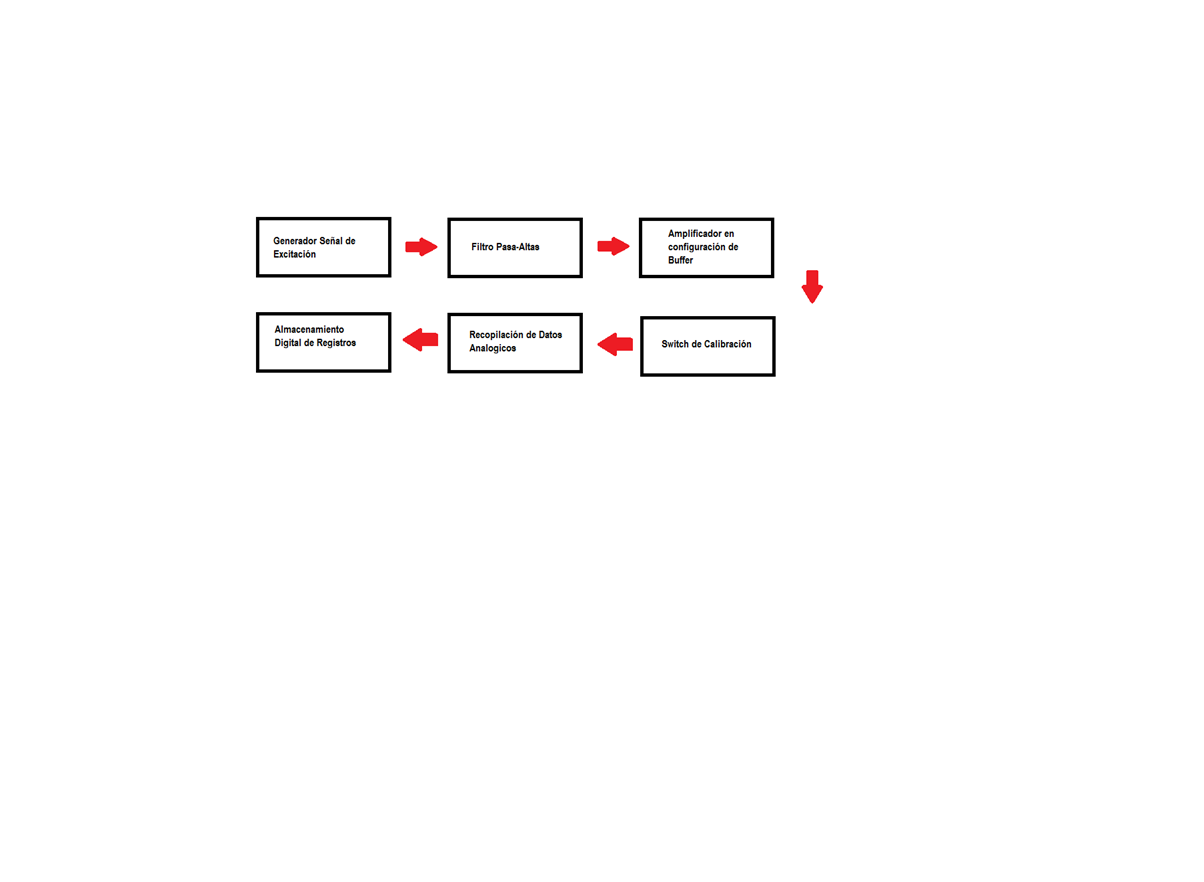
\includegraphics[width=0.5\textwidth]{./Imagenes/Diagrama de Bloques.png}
					\caption{Diagrama de BLoques para el circuito de Bioimpedanciometría}
				\end{figure}
			
					\subparagraph{Generador de Señal de Excitación}
					\hfill\break
En primer lugar se encuentra la etapa generadora de señales, que produce la onda de excitación la cual posteriormente se aplicara sobre el tejido involucrado en el proceso de sensado de bioimpedancia. Para efecto de tal fin, el circuito integrado AD5933 utiliza un DDS o integrado de Síntesis Digital Directa, que a partir de una señal de reloj de referencia produce para este particular caso frecuencias de alrededor de 100 KHz. Adicionalmente es prudente mencionar que la naturaleza de las señales generadas es digital, y de las señales aplicadas sobre la impedancia desconocida es analógica, lo que por ende  implica emplear un DAC o Convertidor de Señales Digitales a Analógicas.
Esta señal, entre tanto, posee un nivel de DC, y este nivel varía entre la etapa de transmisión y recepción   por lo cual es posible que se produzca inexactitud en el dato recopilado consecuencia de la diferencia de polarización, de manera que la señal debe ser tratada en búsqueda de disminuir este efecto. 

					\subparagraph{Filtro Pasa-Altas}
					\hfill\break
Para efecto de una señal más “limpia” que permita su procesamiento apropiado se  realiza un filtro con frecuencia de corte cercana a cero, de manera que se elimine el componente de DC que trae la onda.											

					\subparagraph{Amplificador en configuración de Buffer}
					\hfill\break
Del mismo modo el IC AD5933 es propenso a verse afectado por corrientes de polarización, tensiones de offset y al Factor de Rechazo de Modo Común o CMRR, en consecuencia  la elección de un amplificador que disminuya tales indeseables características implica un mejor rendimiento. Conjuntamente a lo ya mencionado, la configuración de Buffer para dicho amplificador permite tener una baja impedancia a la salida y ayudar así a disminuir el margen de error que pueda ser perceptible en la bioimpedancia tratada.				

					\subparagraph{Switch de Calibración}
					\hfill\break
En esta sección del circuito, la secuencia seguida es una recomendación del fabricante, la cual consiste en cambiar de posición un switch ubicado en la salida de transmisión del sistema, o lo que es igual, donde es emitida la señal de excitación que pasara sobre la carga, colocando una resistencia de calibración que le indicara al circuito una escala restringida de impedancias (en nuestro caso entre 100Ω y 1KΩ), para posteriormente tomar el dato de impedancia desconocido y traducirlo en información procesable con la cual se hará más adelante el control de potencia.				
				
					\subparagraph{Recopilación de Datos Analógicos}
					\hfill\break				
Una vez se ha reducido al máximo las posibles variaciones que podrían representar inexactitudes o datos erróneos, tanto externos al circuito como internos a este, la recopilación de datos hace plausible la modificación de la ganancia, en búsqueda de obtener una señal siempre legible e interpretable por el Procesador de Señal Digital o DSP del integrado. Previo a este procesamiento, es claro mencionar que la señal debe pasar por un ADC  o convertidor de Analógico a Digital para poder ingresar al DSP.   

					\subparagraph{Almacenamiento Digital de Registros}
					\hfill\break
Para el momento en el que ingresa la señal con la información recopilada al DSP, estos datos ya son digitales y se realiza una Transformada de Fourier Discreta, DFT, con la cual se extrae el valor imaginario y el valor real de la bioimpedancia evaluada. Como muchos de los parámetros que establece el AD5933, el almacenamiento de tales datos reales e imaginarios es mediante registros y son estos registros los que el microcontrolador gestionara en el control de potencia.				

				\paragraph{Pautas Establecidas }
				\hfill\break								
Como se mencionó con anterioridad, la bioimpedancia es un valor dependiente de la frecuencia pues se ve afectada ante un cambio de esta, por lo tanto, es prudente realizar con el IC AD5933 un barrido en frecuencia que permita saber el comportamiento de tal impedancia y no solo su valor puntual en un punto específico del espectro. 
Adicional a esto en procura de no generar una respuesta motora en el paciente, la gama de frecuencias superiores o iguales a 100KHz, limita o elimina por completo cualquier efecto perjudicial sobre un organismo vivo. 
Por último la recopilación sucesiva de datos pretende estimar un ponderado que se acerque al valor real de la bioimpedancia, con el fin de no desperdiciar o carecer de potencia en la salida del electrobisturí. 

			\subsubsection{Características}
Previamente se realizó una breve explicación sobre el papel que cumple, dentro de los subcircuitos, los elementos usados para el sistema de bioimpedanciometría. Por lo tanto, a continuación se pretende entrar en detalle acerca del rol de dichos subcircuitos en proceso de toma de datos y su posterior análisis.  

				\paragraph{Componentes}
				\hfill\break
Para un contexto más general el circuito de Bioimpedanciometría cumple varios roles fundamentales en la lógica del sistema completo,  y su propósito se dividirá en secciones  para su comprensión global.
Para todos los procesos que se enlistaran posteriormente, el tratamiento de datos sigue, en principio, el mismo ciclo, la diferencia entre estos es el uso final de la información obtenida.
De acuerdo a lo mencionado el circuito integrado AD5933 almacena internamente los valores de los registros real e imaginario una vez finalizado cada periodo de sensado, siendo que cada nuevo senso sobre una cierta impedancia, refresca o cambia el dato almacenado en tales registros.
Una vez la totalidad de los datos sean enviados por el método de I²C  del IC al procesador de propósito general, en este caso el Atmega328-PA sabemos no solo por lo dado en la hoja de datos del AD5933 [6], sino también por lo analizado teóricamente en diversos textos [8], que:
$$Z = X + jY; ó Z = r \angle \Theta;$$								
			




\end{document}